\section{Desarrollo}
	
	\section{Fuentes de origen de alimentación de los sistemas trifásicos}
	
	Los sistemas trifásicos se emplean ampliamente en instalaciones industriales y de potencia debido a que permiten transmitir energía de manera más uniforme que los sistemas monofásicos. En una alimentación trifásica balanceada, las tres tensiones tienen la misma magnitud y frecuencia, pero se encuentran desfasadas entre sí \(120^{\circ}\). Esta separación angular hace que la suma instantánea de potencias sea prácticamente constante cuando la carga está equilibrada.
	
	\subsection{Transformadores trifásicos}
	
	Una de las fuentes principales de alimentación trifásica es el transformador trifásico. Este equipo puede construirse como una sola unidad con tres columnas magnéticas, o bien mediante la conexión de tres transformadores monofásicos. Su función principal es modificar el nivel de tensión de un sistema de corriente alterna, manteniendo la frecuencia de operación.
	
	El transformador está constituido por dos partes fundamentales:
	
	\begin{itemize}[leftmargin=1.2cm]
		\item \textbf{Núcleo magnético:} formado por láminas ferromagnéticas, normalmente de acero al silicio, que proporcionan una trayectoria de baja reluctancia para el flujo magnético. La laminación reduce las pérdidas por corrientes parásitas.
		\item \textbf{Bobinados o devanados:} conductores enrollados alrededor del núcleo. El devanado primario recibe energía de la fuente y el devanado secundario entrega energía a la carga.
	\end{itemize}
	
	\begin{figure}[H]
		\centering
		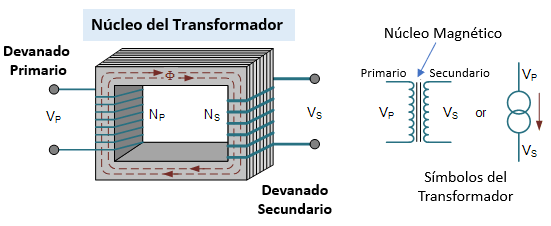
\includegraphics[width=0.62\textwidth]{assets/img/1.png}
		\caption{Núcleo y devanados de un transformador.}
	\end{figure}
	
	\subsection{Principio de operación}
	
	El funcionamiento del transformador se basa en la inducción electromagnética. Al aplicar una tensión alterna al devanado primario, circula una corriente que produce un flujo magnético variable en el núcleo. Dicho flujo enlaza al devanado secundario e induce una tensión alterna. La relación ideal entre tensiones y número de espiras se expresa como:
	
	\begin{equation}
		\frac{V_1}{V_2}=\frac{N_1}{N_2},
	\end{equation}
	
	donde \(V_1\) y \(V_2\) son las tensiones primaria y secundaria, mientras que \(N_1\) y \(N_2\) son los números de espiras correspondientes. Si \(N_2>N_1\), el transformador es elevador; si \(N_2<N_1\), es reductor.
	
	\subsection{Configuraciones para sistemas trifásicos}
	
	Las conexiones más utilizadas en transformadores trifásicos son estrella y delta. En la conexión estrella \((Y)\), un extremo de cada devanado se conecta a un punto común llamado neutro. Esta configuración permite obtener tensión de línea y tensión de fase, por lo que resulta útil para alimentar cargas trifásicas y monofásicas. En la conexión delta \((\Delta)\), los devanados se conectan formando un lazo cerrado, de manera que cada bobina queda entre dos líneas del sistema.
	
	Las combinaciones típicas son:
	
	\begin{itemize}[leftmargin=1.2cm]
		\item \textbf{Y--Y:} útil cuando se requiere neutro en ambos lados y conexión a tierra.
		\item \textbf{\(\Delta\)--\(\Delta\):} común en cargas industriales donde no se requiere conductor neutro.
		\item \textbf{Y--\(\Delta\) y \(\Delta\)--Y:} usadas para adaptar niveles de tensión en transmisión y distribución, además de proporcionar desplazamientos de fase útiles para ciertos sistemas.
	\end{itemize}
	
	\begin{figure}[H]
		\centering
		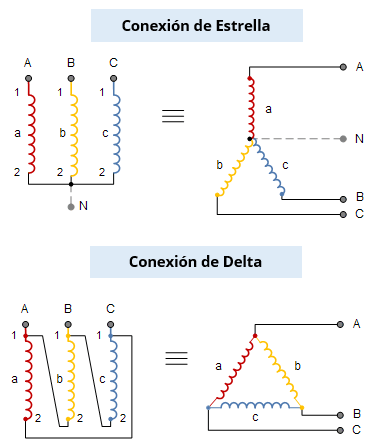
\includegraphics[width=0.5\textwidth]{assets/img/2.png}
		\caption{Configuraciones de transformadores trifásicos.}
	\end{figure}
	
	% ------------------------------------------------------------
	% Sección 2
	% ------------------------------------------------------------
	\section{Potencia eléctrica. Excitación sinusoidal en elementos pasivos R, L y C}
	
	En corriente alterna, la tensión y la corriente son funciones del tiempo. La potencia instantánea se define como el producto entre ambas magnitudes:
	
	\begin{equation}
		p(t)=v(t)i(t).
	\end{equation}
	
	Cuando \(p(t)>0\), la carga absorbe energía de la fuente; cuando \(p(t)<0\), parte de la energía almacenada en los campos eléctricos o magnéticos regresa a la fuente. Este intercambio es la causa de la potencia reactiva en elementos inductivos y capacitivos.
	
	\subsection{Carga resistiva}
	
	En una carga puramente resistiva, tensión y corriente están en fase:
	
	\begin{equation}
		v(t)=V_m\sin(\omega t), \qquad i(t)=I_m\sin(\omega t).
	\end{equation}
	
	Por tanto,
	
	\begin{equation}
		p(t)=V_mI_m\sin^2(\omega t)=\frac{V_mI_m}{2}\left[1-\cos(2\omega t)\right].
	\end{equation}
	
	La potencia instantánea nunca es negativa y su valor medio corresponde a la potencia activa. Como no existe desfase, el factor de potencia es unitario.
	
	\subsection{Carga inductiva}
	
	En una carga inductiva ideal, la corriente se retrasa \(90^{\circ}\) respecto a la tensión:
	
	\begin{equation}
		i(t)=I_m\sin\left(\omega t-\frac{\pi}{2}\right).
	\end{equation}
	
	La potencia instantánea queda:
	
	\begin{equation}
		p(t)=-\frac{V_mI_m}{2}\sin(2\omega t).
	\end{equation}
	
	El valor medio en un ciclo es cero para el elemento ideal, ya que la energía se almacena temporalmente en el campo magnético y después se devuelve a la fuente. En cargas reales, como motores y transformadores, también existe resistencia, por lo que hay una componente activa y una componente reactiva inductiva.
	
	\subsection{Carga capacitiva}
	
	En una carga capacitiva ideal, la corriente se adelanta \(90^{\circ}\) respecto a la tensión. El comportamiento también produce intercambio de energía con la fuente, pero ahora asociado al campo eléctrico. La potencia reactiva capacitiva se considera de signo contrario a la inductiva, por lo que puede emplearse para compensar cargas inductivas.
	
	\subsection{Potencia activa, reactiva y aparente}
	
	Para señales sinusoidales, si la tensión eficaz es \(V\), la corriente eficaz es \(I\) y el ángulo de desfase es \(\varphi\), se definen:
	
	\begin{align}
		P &= VI\cos\varphi && \text{potencia activa [W]},\\
		Q &= VI\sin\varphi && \text{potencia reactiva [VAR]},\\
		S &= VI && \text{potencia aparente [VA]}.
	\end{align}
	
	La potencia activa representa la energía transformada en trabajo útil, calor o luz. La potencia reactiva representa energía alternadamente almacenada y devuelta por elementos reactivos. La potencia aparente es la demanda total que observa la fuente.
	
	En forma compleja:
	
	\begin{equation}
		\mathbf{S}=\mathbf{V}\mathbf{I}^{*}=P+jQ,
	\end{equation}
	
	con magnitud:
	
	\begin{equation}
		|\mathbf{S}|=\sqrt{P^2+Q^2}.
	\end{equation}
	
	\subsection{Triángulo de potencias}
	
	La relación entre \(P\), \(Q\) y \(S\) se representa con el triángulo de potencias. El ángulo \(\varphi\) indica el desfase entre tensión y corriente, y su coseno define el factor de potencia:
	
	\begin{equation}
		FP=\cos\varphi=\frac{P}{S}.
	\end{equation}
	
	\begin{figure}[H]
		\centering
		\begin{subfigure}{0.8\textwidth}
			\centering
			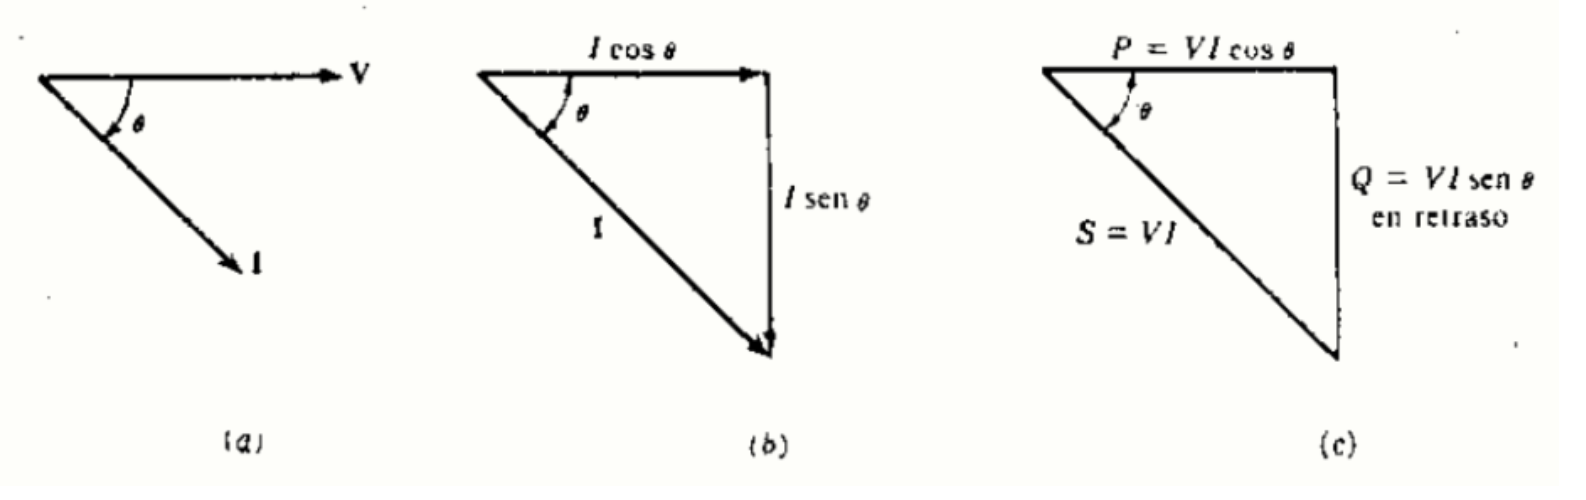
\includegraphics[width=\textwidth]{assets/img/3a.png}
			\caption{Carga inductiva.}
		\end{subfigure}
		
		\begin{subfigure}{0.8\textwidth}
			\centering
			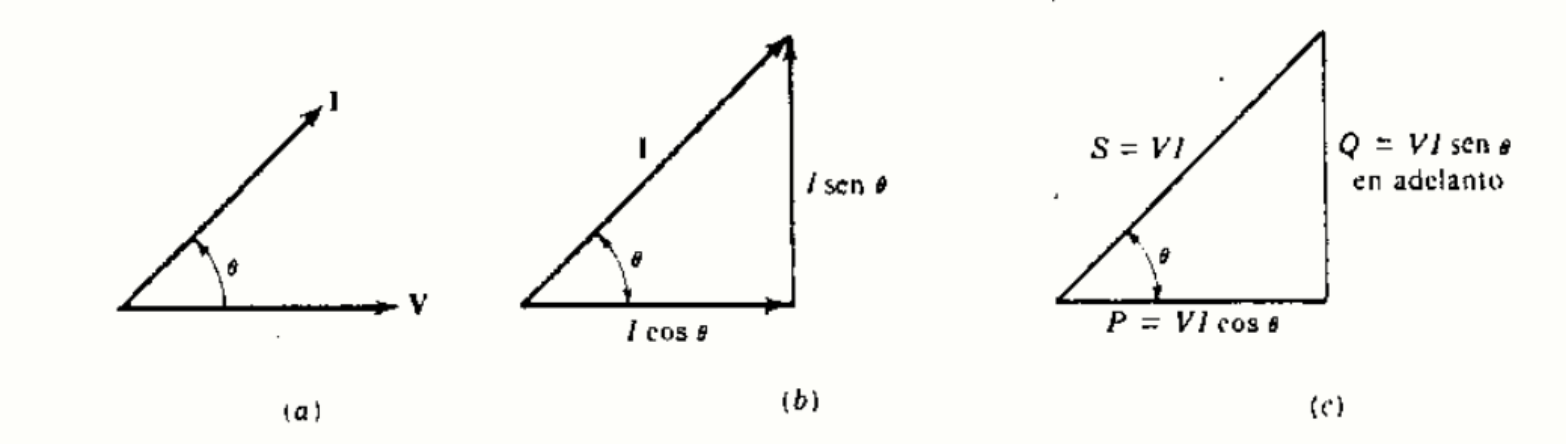
\includegraphics[width=\textwidth]{assets/img/3b.png}
			\caption{Carga capacitiva.}
		\end{subfigure}
		\caption{Triángulos de potencias.}
	\end{figure}
	
	\subsection{Potencia trifásica}
	
	En un sistema trifásico balanceado, la potencia total puede calcularse como:
	
	\begin{align}
		P_T &= \sqrt{3}V_LI_L\cos\varphi,\\
		Q_T &= \sqrt{3}V_LI_L\sin\varphi,\\
		S_T &= \sqrt{3}V_LI_L.
	\end{align}
	
	Cuando el sistema no está completamente balanceado, es preferible sumar las potencias de cada fase:
	
	\begin{align}
		P_T &= P_A+P_B+P_C,\\
		Q_T &= Q_A+Q_B+Q_C,\\
		S_T &\approx S_A+S_B+S_C.
	\end{align}
	
	\subsection{Análisis experimental de carga resistiva en configuración estrella}
	
	En la configuración estrella se conectaron cargas resistivas de forma que cada fase quedara alimentada respecto al punto común. Los resultados registrados se muestran en la Tabla \ref{tab:estrella}. La potencia reactiva fue muy pequeña en comparación con la activa, lo que confirma que la carga se comportó principalmente como resistiva.
	
	\begin{table}[H]
		\centering
		\caption{Mediciones en configuración estrella.}
		\label{tab:estrella}
		
			\begin{tabular}{c c c c c c c c}
				\toprule
				Fase & \(I\) [A] & \(V\) [V] & \(S\) [VA] & \(P\) [W] & \(Q\) [VAR] & \(\theta\) [\(^\circ\)] & \(FP\) \\
				\midrule
				A & 1.612 & 125.6 & 201 & 201 & 7 & 0.2 & 1.00 \\
				B & 1.633 & 126.3 & 206 & 201 & 0 & 0.2 & 1.00 \\
				C & 1.570 & 125.1 & 197 & 201 & 6 & 0.2 & 1.00 \\
				\bottomrule
		\end{tabular}
	\end{table}
	
	La suma de potencias activas fue aproximadamente \(P_T=603\unit{W}\), mientras que la potencia reactiva total fue cercana a \(13\unit{VAR}\). Esto indica que el factor de potencia global estuvo prácticamente en la unidad y que la potencia aparente se destinó casi por completo a potencia útil.
	
	\subsection{Análisis experimental de carga resistiva en configuración delta}
	
	En la configuración delta, cada carga quedó conectada entre dos líneas. Los valores de tensión fueron mayores que en estrella, por lo que también aumentaron las corrientes y las potencias por rama. Los resultados se presentan en la Tabla \ref{tab:delta}.
	
	\begin{table}[H]
		\centering
		\caption{Mediciones en configuración delta.}
		\label{tab:delta}
			\begin{tabular}{c c c c c c c c}
				\toprule
				Rama & \(I\) [A] & \(V\) [V] & \(S\) [VA] & \(P\) [W] & \(Q\) [VAR] & \(\theta\) [\(^\circ\)] & \(FP\) \\
				\midrule
				AB & 2.119 & 216.4 & 459 & 459 & 15 & 0.2 & 1.00 \\
				BC & 2.180 & 216.5 & 473 & 473 & 0 & 0.2 & 1.00 \\
				CA & 2.161 & 214.8 & 464 & 464 & 12 & 0.2 & 1.00 \\
				\bottomrule
		\end{tabular}
	\end{table}
	
	La potencia activa total fue aproximadamente \(P_T=1396\unit{W}\), con potencia reactiva pequeña respecto a la activa. Esto confirma nuevamente el comportamiento resistivo de la carga y permite comparar cómo la conexión delta demanda mayor potencia bajo la misma fuente de alimentación.
	
	% ------------------------------------------------------------
	% Sección 3
	% ------------------------------------------------------------
	\section{Factor de potencia y su corrección}
	
	El factor de potencia indica qué proporción de la potencia aparente se convierte en potencia activa. Se define como:
	
	\begin{equation}
		FP=\frac{P}{S}=\cos\varphi.
	\end{equation}
	
	Un \(FP\) cercano a 1 significa que la corriente está casi en fase con la tensión y que la energía se aprovecha de manera eficiente. Un \(FP\) bajo indica una corriente mayor para entregar la misma potencia activa, debido a que existe una componente reactiva considerable.
	
	\begin{figure}[H]
		\centering
		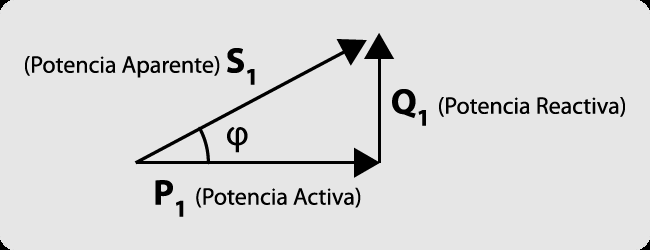
\includegraphics[width=0.55\textwidth]{assets/img/page10_img01.png}
		\caption{Relación entre potencia activa, reactiva y aparente para definir el factor de potencia.}
		\label{fig:fp_triangulo}
	\end{figure}
	
	\subsection{Interpretación física del factor de potencia}
	
	En una carga resistiva ideal, \(\varphi=0^{\circ}\), por lo que \(FP=1\). En una carga inductiva, la corriente se retrasa respecto a la tensión y se considera potencia reactiva positiva. En una carga capacitiva, la corriente se adelanta respecto a la tensión y la potencia reactiva tiene signo contrario a la inductiva. Por esta razón, un banco de capacitores puede compensar una carga predominantemente inductiva, como un motor.
	
	El ángulo \(\varphi\) también puede entenderse a partir del triángulo de impedancias:
	
	\begin{equation}
		Z=R+j(X_L-X_C),
	\end{equation}
	
	por lo que:
	
	\begin{equation}
		\varphi=\tan^{-1}\left(\frac{X_L-X_C}{R}\right).
	\end{equation}
	
	\begin{figure}[H]
		\centering
		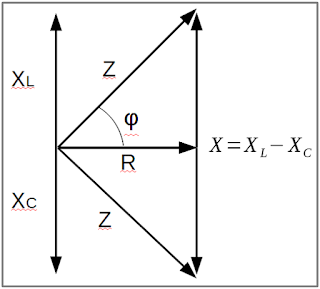
\includegraphics[width=0.4\textwidth]{assets/img/page14_img01.png}
		\caption{Triángulo de impedancias para una carga con resistencia, reactancia inductiva y reactancia capacitiva.}
		\label{fig:triangulo_impedancias}
	\end{figure}
	
	Las reactancias inductiva y capacitiva dependen de la frecuencia angular \(\omega=2\pi f\):
	
	\begin{align}
		X_L &= \omega L,\\
		X_C &= \frac{1}{\omega C}.
	\end{align}
	
	\begin{figure}[H]
		\centering
		\begin{subfigure}{0.4\textwidth}
			\centering
			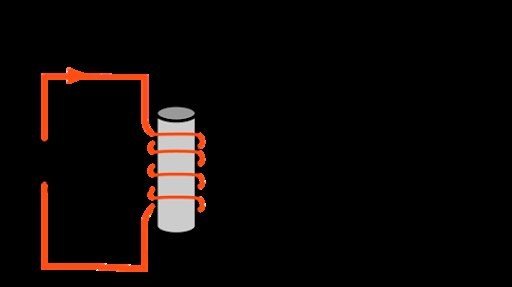
\includegraphics[width=\textwidth]{assets/img/page14_img02.png}
			\caption{Reactancia inductiva.}
		\end{subfigure}\hfill
		\begin{subfigure}{0.4\textwidth}
			\centering
			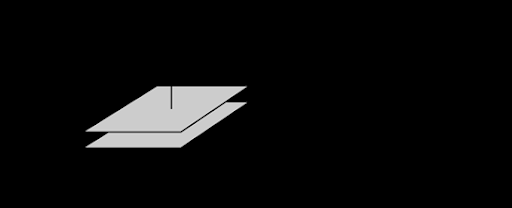
\includegraphics[width=\textwidth]{assets/img/page14_img03.png}
			\caption{Reactancia capacitiva.}
		\end{subfigure}
		\caption{Comportamiento de corriente y tensión en elementos reactivos.}
		\label{fig:reactancias}
	\end{figure}
	
	\subsection{Corrección del factor de potencia}
	
	Corregir el factor de potencia consiste en reducir la componente reactiva vista por la fuente. Para una carga inductiva, se coloca una capacitancia en paralelo, de modo que la potencia reactiva capacitiva compense parte de la potencia reactiva inductiva:
	
	\begin{equation}
		Q_{nuevo}=Q_L-Q_C.
	\end{equation}
	
	Si se desea pasar de un ángulo inicial \(\varphi_1\) a un ángulo final \(\varphi_2\), la potencia reactiva que debe aportar el banco de capacitores es:
	
	\begin{equation}
		Q_C=P\left(\tan\varphi_1-\tan\varphi_2\right).
	\end{equation}
	
	Para un banco trifásico conectado en estrella:
	
	\begin{equation}
		C_Y=\frac{Q_C}{3\omega V_F^2},
	\end{equation}
	
	mientras que para conexión delta:
	
	\begin{equation}
		C_{\Delta}=\frac{Q_C}{3\omega V_L^2}.
	\end{equation}
	
	La corrección no busca eliminar por completo la potencia reactiva en todos los casos, sino reducirla hasta obtener un factor de potencia adecuado y evitar sobrecompensación capacitiva.
	
	\subsection{Montaje experimental de referencia}
	
	A continuación se muestran las imágenes empleadas desde la sección de factor de potencia y corrección, tomadas como referencia visual del montaje y del equipo utilizado.
	
	\begin{figure}[H]
		\centering
		\begin{subfigure}{0.45\textwidth}
			\centering
			\rotatebox{90}{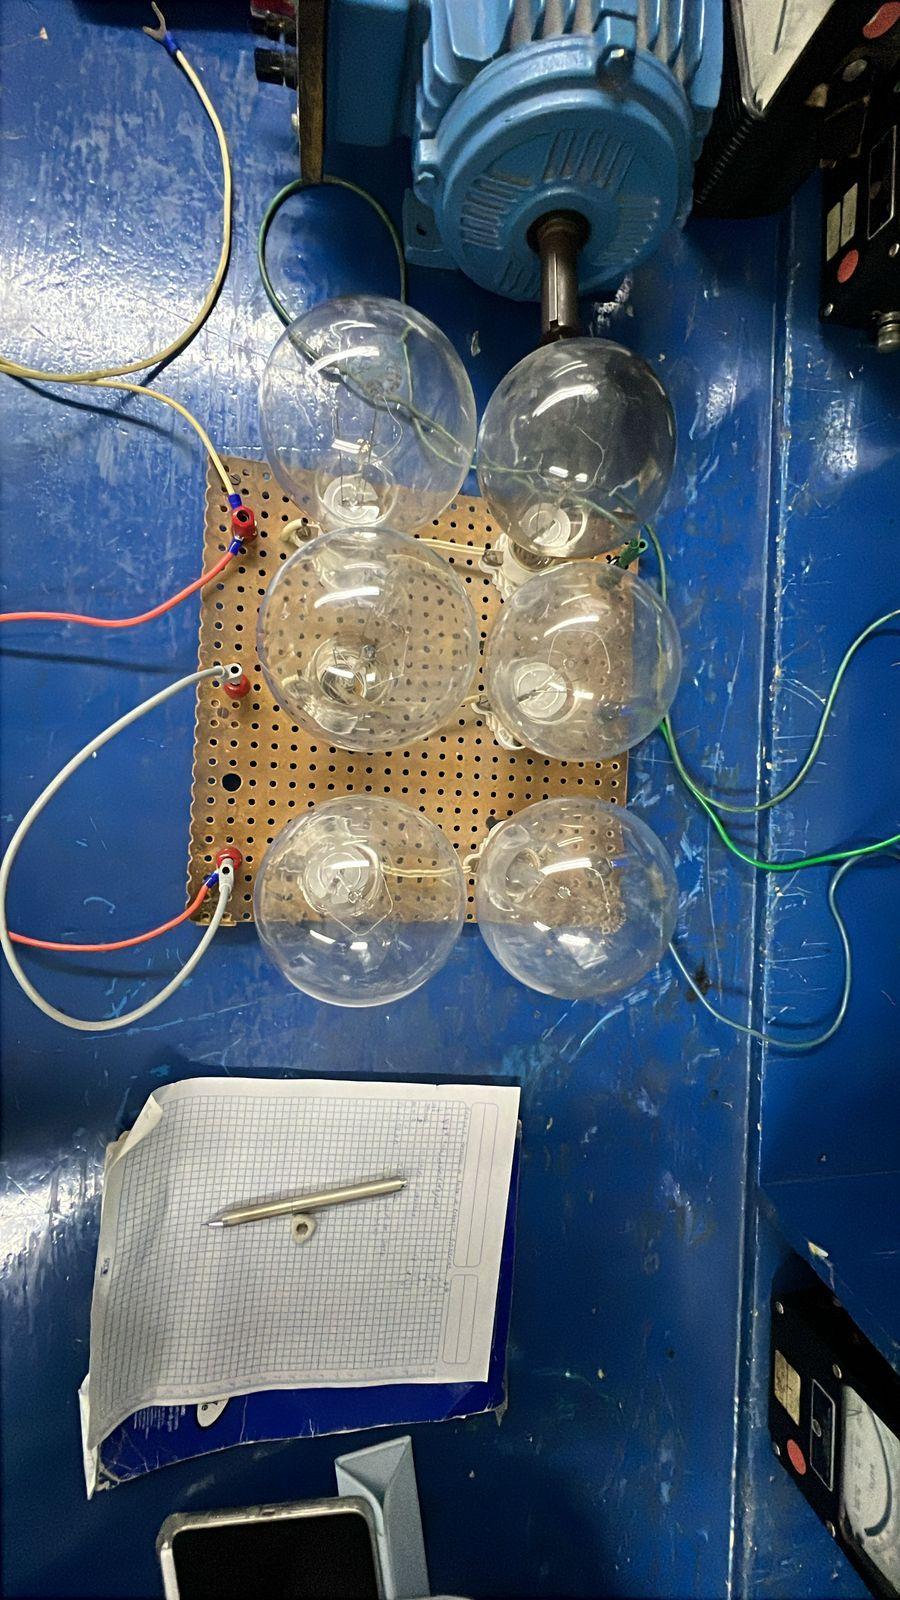
\includegraphics[height=7cm]{assets/img/page16_img01.png}}
			\caption{Montaje de carga resistiva en estrella.}
		\end{subfigure}\hfill
		\begin{subfigure}{0.50\textwidth}
			\centering
			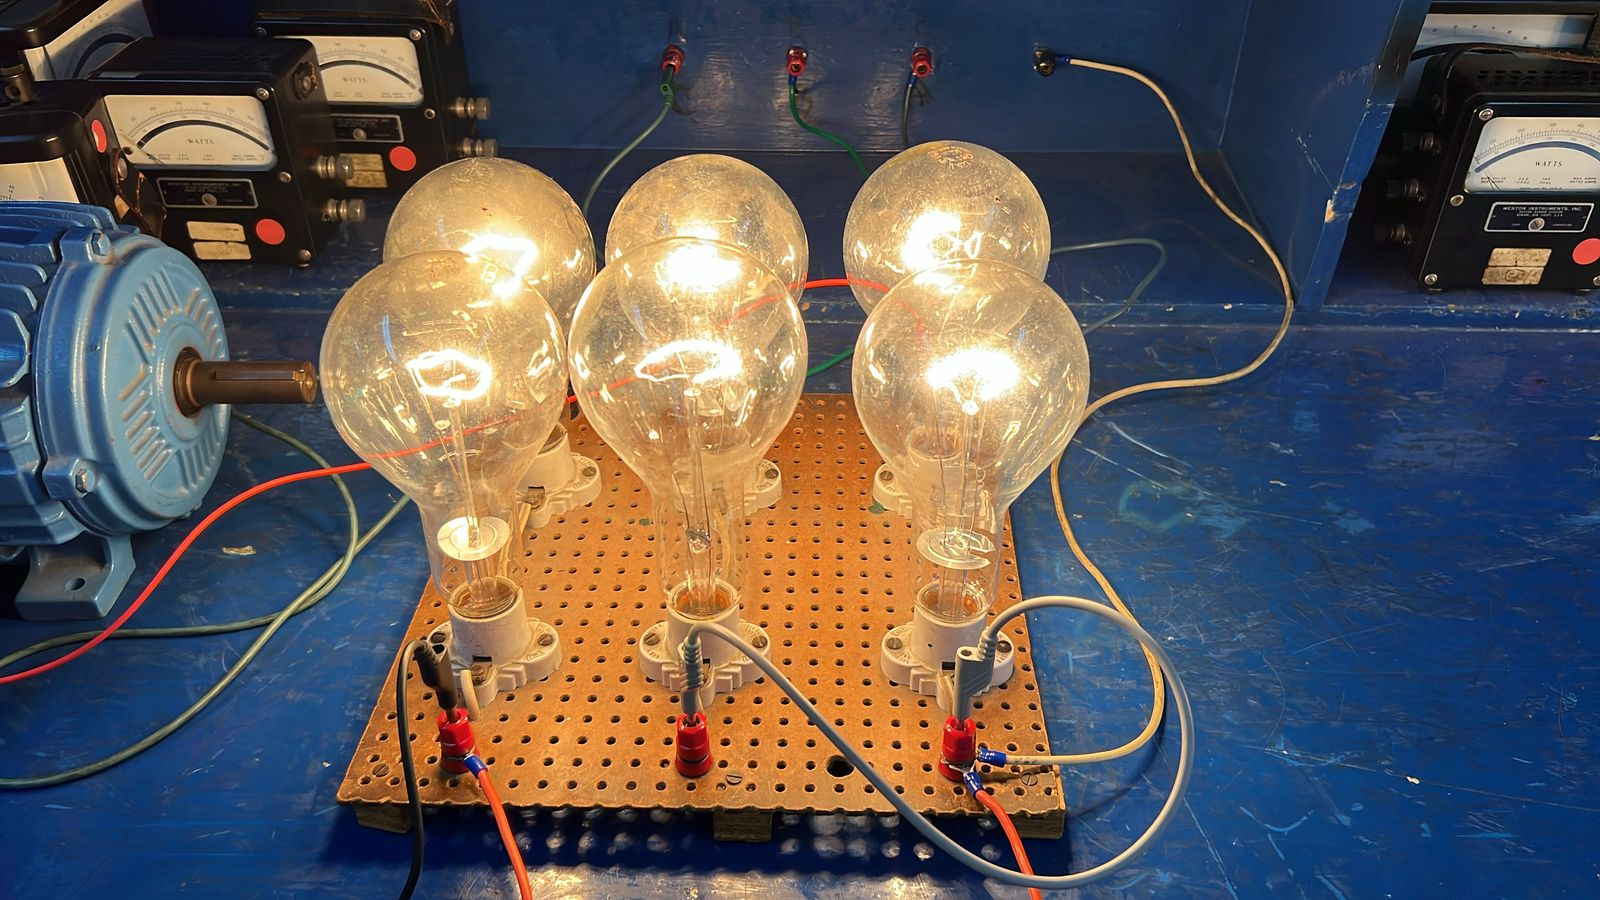
\includegraphics[height=4cm]{assets/img/page16_img02.png}
			\caption{Medición en configuración estrella.}
		\end{subfigure}
		\caption{Evidencia de la conexión en estrella.}
		\label{fig:estrella_fotos}
	\end{figure}
	
	\begin{figure}[H]
		\centering
		\begin{subfigure}{0.45\textwidth}
			\centering
			\includegraphics[height=4cm]{assets/img/page17_img01.png}
			\caption{Medición de corriente en delta.}
		\end{subfigure}\hfill
		\begin{subfigure}{0.50\textwidth}
			\centering
			\includegraphics[height=4cm]{assets/img/page17_img02.png}
			\caption{Montaje de carga resistiva en delta.}
		\end{subfigure}
		\caption{Evidencia de la conexión en estrella.}
	\end{figure}
	
	\begin{figure}[H]
		\centering
		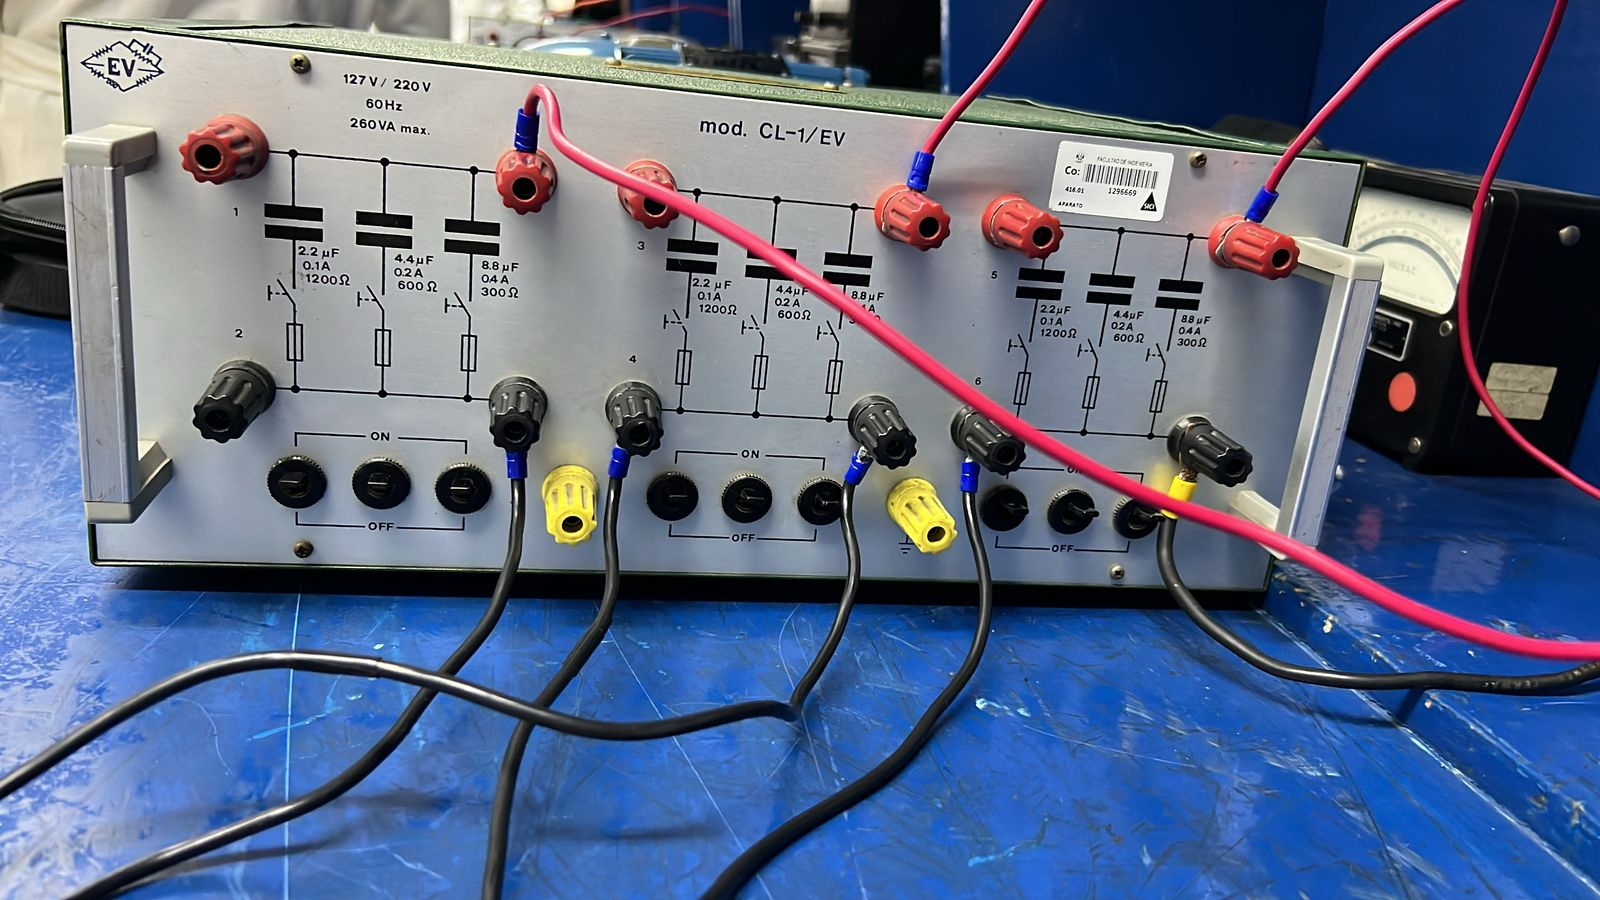
\includegraphics[width=0.7\textwidth]{assets/img/page18_img01.png}
		\caption{Banco de capacitores utilizado para la corrección del factor de potencia.}
		\label{fig:banco_capacitores}
	\end{figure}
	
	\subsection{Medición del motor sin banco de capacitores}
	
	Primero se analizó la carga del motor sin conectar el banco de capacitores. Los valores registrados se presentan en la Tabla \ref{tab:motor_sin_cap}. Se observa que la potencia reactiva es casi igual a la potencia aparente, lo cual indica un ángulo de desfase elevado y un bajo factor de potencia.
	
	\begin{figure}[H]
		\centering
		\begin{subfigure}{0.48\textwidth}
			\centering
			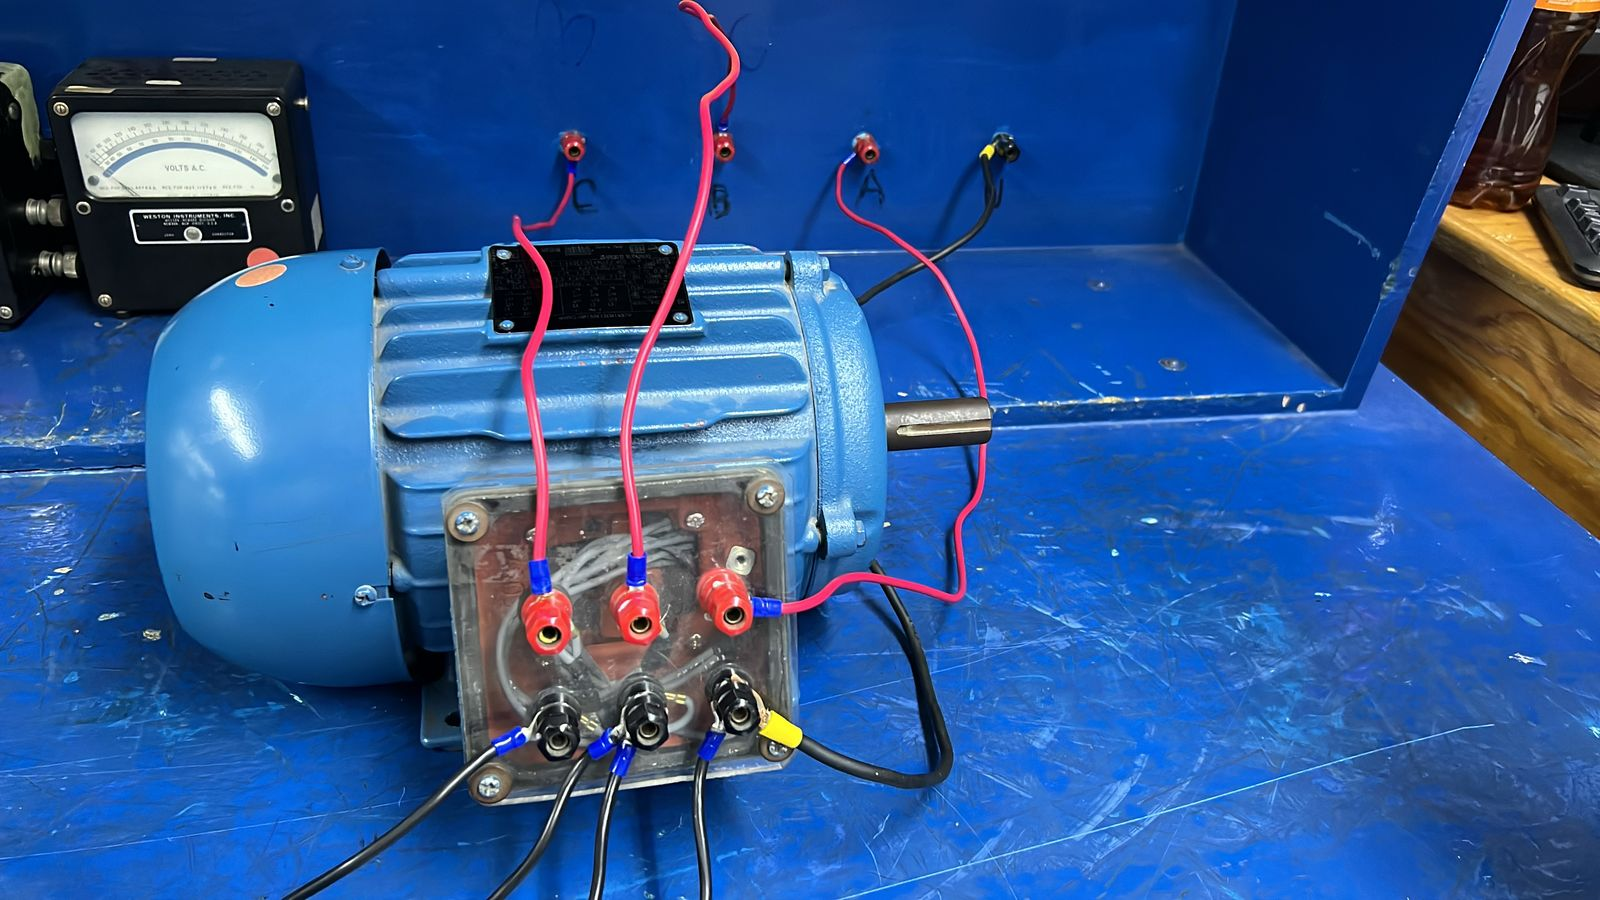
\includegraphics[width=\textwidth]{assets/img/page19_img01.png}
			\caption{Motor conectado sin compensación.}
		\end{subfigure}\hfill
		\begin{subfigure}{0.32\textwidth}
			\centering
			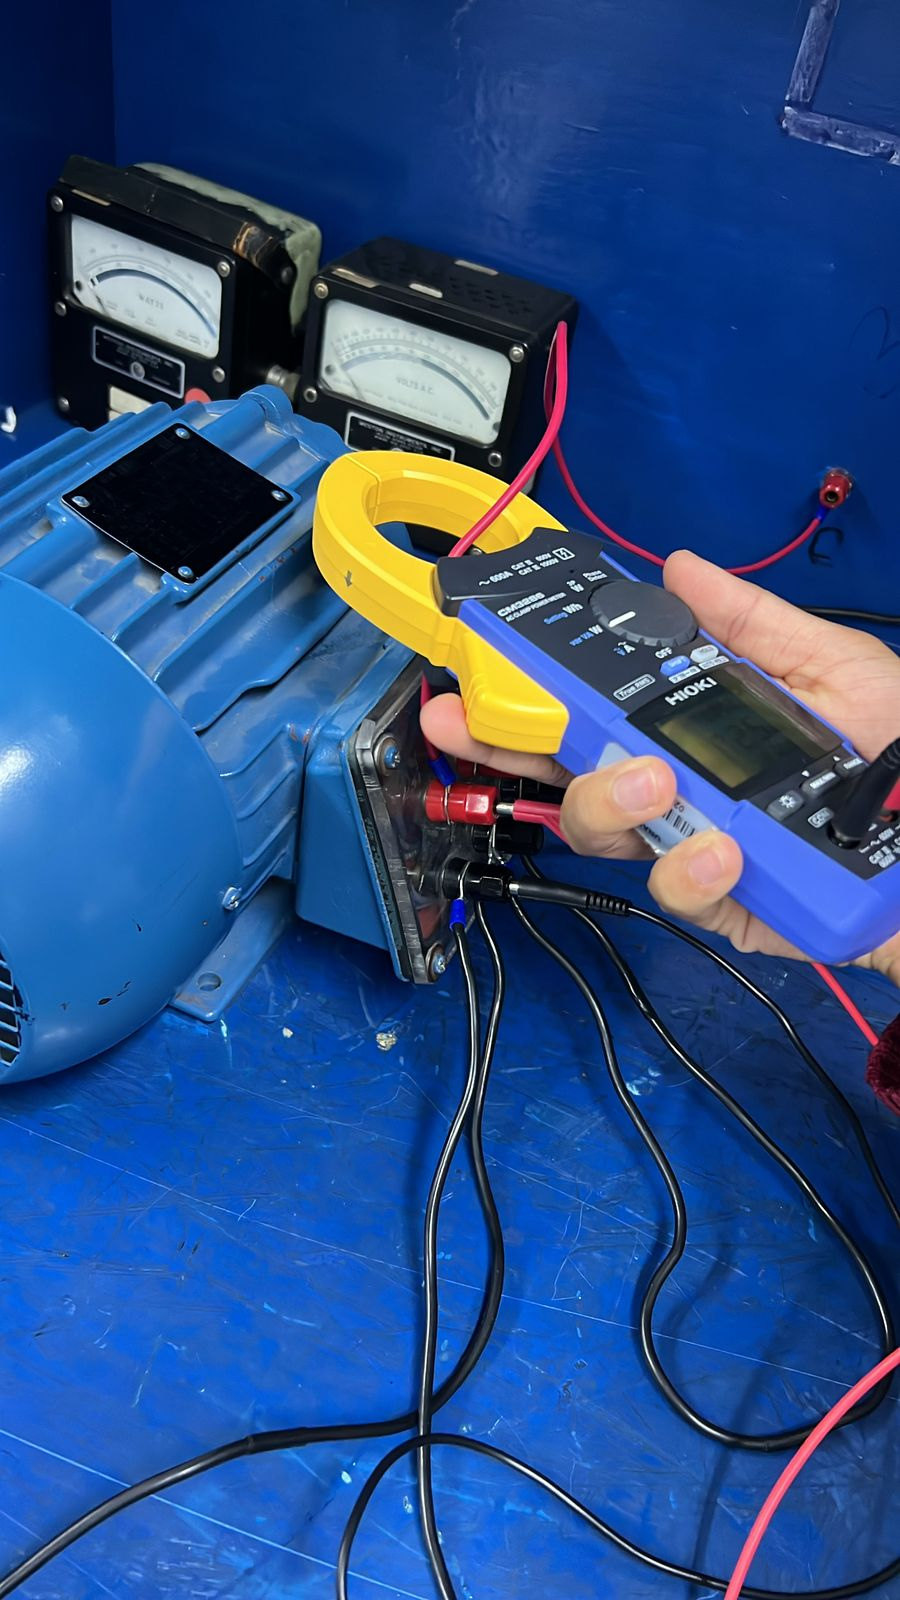
\includegraphics[height=5.0cm]{assets/img/page19_img02.png}
			\caption{Medición de corriente.}
		\end{subfigure}
		\caption{Carga del motor sin banco de capacitores.}
		\label{fig:motor_sin_cap}
	\end{figure}
	
	\begin{table}[H]
		\centering
		\caption{Mediciones del motor sin capacitores en la entrada.}
		\label{tab:motor_sin_cap}
			\begin{tabular}{c c c c c c c c}
				\toprule
				Fase & \(I\) [A] & \(V\) [V] & \(S\) [VA] & \(P\) [W] & \(Q\) [VAR] & \(\theta\) [\(^\circ\)] & \(FP\) \\
				\midrule
				A & 2.183 & 125.6 & 273 & 20 & 272 & 85.9 & 0.073 \\
				B & 2.269 & 126.7 & 287 & 30 & 285 & 85.6 & 0.105 \\
				C & 2.253 & 126.1 & 285 & 24 & 284 & 84.7 & 0.084 \\
				\bottomrule
		\end{tabular}
	\end{table}
	
	\subsection{Medición con banco de capacitores conectado}
	
	Posteriormente se conectó el banco de capacitores al mismo sistema de alimentación. La Tabla \ref{tab:motor_con_cap} resume los valores empleados para el análisis. En esta condición la potencia aparente total disminuyó respecto a la condición sin capacitores, lo que indica que la fuente entregó menor corriente para una carga con compensación reactiva.
	
	\begin{figure}[H]
		\centering
		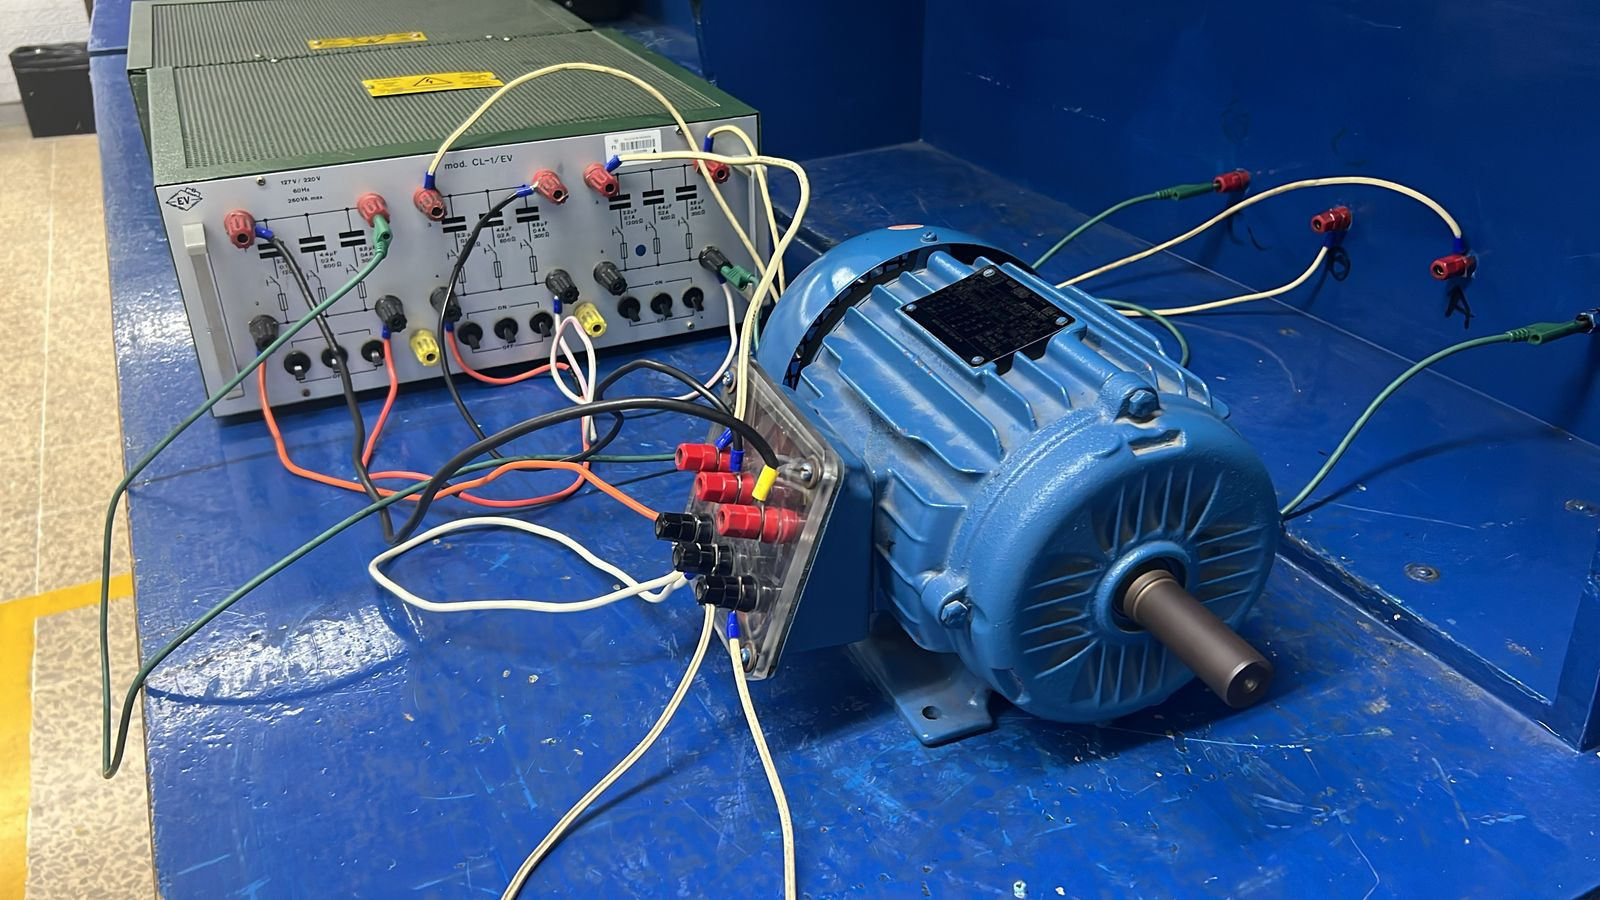
\includegraphics[width=0.7\textwidth]{assets/img/page20_img01.png}
		\caption{Motor operando con banco de capacitores conectado.}
		\label{fig:motor_con_cap}
	\end{figure}
	
	\begin{table}[H]
		\centering
		\caption{Mediciones con banco de capacitores conectado.}
		\label{tab:motor_con_cap}
			\begin{tabular}{c c c c c c c c}
				\toprule
				Fase & \(I\) [A] & \(V\) [V] & \(S\) [VA] & \(P\) [W] & \(Q\) [VAR] & \(\theta\) [\(^\circ\)] & \(FP\) \\
				\midrule
				A & 1.530 & 126.0 & 192 & 21 & 191 & 81.7 & 0.100 \\
				B & 1.522 & 125.8 & 192 & -& 190 & 82.7 & 0.111 \\
				C & 2.167 & 126.3 & 274 & - & 271 & 85.2 & 0.097 \\
				\bottomrule
		\end{tabular}
	\end{table}
	
	\textit{Nota:} en las lecturas registradas para las fases B y C con banco de capacitores, la potencia activa debe verificarse contra el instrumento de medición, ya que el valor de \(FP\) y la potencia aparente sugieren que la potencia activa real es mucho menor que la aparente.
	
	\subsection{Comparación: motor aislado y motor con banco de capacitores}
	
	Para verificar la influencia del factor de potencia en el consumo de corriente, se compararon los valores promedio de corriente y la suma de potencia aparente antes y después de conectar el banco de capacitores.
	
	\begin{table}[H]
		\centering
		\caption{Comparación global de la carga del motor.}
		\label{tab:comparacion_motor}
			\begin{tabular}{l c c c c c}
				\toprule
				Condición & \(I_A\) [A] & \(I_B\) [A] & \(I_C\) [A] & \(I_{prom}\) [A] & \(S_T\) [VA] \\
				\midrule
				Motor sin capacitores & 2.183 & 2.269 & 2.253 & 2.235 & 845 \\
				Motor con banco de capacitores & 1.530 & 1.522 & 2.167 & 1.740 & 658 \\
				\bottomrule
		\end{tabular}
	\end{table}
	
	La disminución promedio de corriente fue:
	
	\begin{equation}
		\Delta I_{prom}=\frac{2.235-1.740}{2.235}\times100\approx22.1\%.
	\end{equation}
	
	Asimismo, la potencia aparente disminuyó de \(845\unit{VA}\) a \(658\unit{VA}\), lo que representa una reducción aproximada de:
	
	\begin{equation}
		\Delta S=\frac{845-658}{845}\times100\approx22.1\%.
	\end{equation}
	
	Con esto se verifica que la corrección del factor de potencia reduce la demanda aparente que debe entregar la fuente. Aunque la potencia activa útil del motor no cambia de forma significativa, la corriente total requerida por el sistema disminuye al compensar parte de la potencia reactiva.
	
	\subsection{Análisis de cargas R, L y C en el mismo sistema de alimentación}
	
	Para completar el análisis se comparó el comportamiento de cargas resistivas, capacitivas e inductivas. La carga resistiva presentó \(FP\approx1\), pues la potencia activa fue prácticamente igual a la potencia aparente. En cambio, las cargas inductiva y capacitiva presentaron bajo factor de potencia, con ángulos cercanos a \(\pm90^{\circ}\).
	
	\begin{table}[H]
		\centering
		\caption{Mediciones para carga capacitiva.}
		\label{tab:carga_capacitiva}
			\begin{tabular}{c c c c c c c c}
				\toprule
				Fase & \(I\) [A] & \(V\) [V] & \(S\) [VA] & \(P\) [W] & \(Q\) [VAR] & \(\theta\) [\(^\circ\)] & \(FP\) \\
				\midrule
				A & 0.675 & 126.0 & 85 & 4 & -85 & -86.4 & 0.054 \\
				B & 0.672 & 126.8 & 87 & 4 & -85 & -87.5 & 0.051 \\
				C & 0.678 & 126.9 & 85 & 6 & -85 & -85.2 & 0.065 \\
				\bottomrule
		\end{tabular}
	\end{table}
	
	\begin{table}[H]
		\centering
		\caption{Mediciones para carga inductiva.}
		\label{tab:carga_inductiva}
			\begin{tabular}{c c c c c c c c}
				\toprule
				Fase & \(I\) [A] & \(V\) [V] & \(S\) [VA] & \(P\) [W] & \(Q\) [VAR] & \(\theta\) [\(^\circ\)] & \(FP\) \\
				\midrule
				A & 2.258 & 125.8 & 284 & 2.9 & 284 & 84.1 & 0.096 \\
				B & 2.270 & 126.3 & 297 & 3.6 & 296 & 85.2 & 0.118 \\
				C & 2.184 & 125.9 & 276 & 2.5 & 275 & 84.3 & 0.095 \\
				\bottomrule
		\end{tabular}
	\end{table}
	
	En la carga capacitiva, el signo negativo de \(Q\) representa potencia reactiva en adelanto. En la carga inductiva, \(Q\) es positiva y la corriente se retrasa respecto a la tensión. Al conectar ambos comportamientos de manera adecuada, la potencia reactiva neta disminuye y el factor de potencia mejora.
	
	\section*{Conclusiones}
	\addcontentsline{toc}{section}{Conclusiones}
	
	Durante la práctica se comprobó que la potencia en corriente alterna no sólo depende de la magnitud de la tensión y la corriente, sino también del desfase entre ambas. En las cargas resistivas conectadas en estrella y delta se obtuvo un factor de potencia cercano a la unidad, ya que la potencia reactiva fue muy pequeña en comparación con la potencia activa. Esto confirma que, en este tipo de carga, casi toda la potencia aparente se aprovecha como potencia útil.
	
	En las cargas inductivas y capacitivas se observó un comportamiento distinto. La corriente quedó desfasada respecto a la tensión, provocando que la potencia reactiva fuera dominante y que el factor de potencia disminuyera. Este efecto es especialmente importante en motores, transformadores y equipos industriales, porque una baja eficiencia en el factor de potencia incrementa la corriente que debe suministrar la fuente.
	
	Al conectar el banco de capacitores al sistema del motor, la potencia aparente total disminuyó de forma apreciable. Con los datos registrados, la corriente promedio pasó de aproximadamente \(2.235\unit{A}\) a \(1.740\unit{A}\), lo que representa una reducción cercana al \(22.1\%\). Por lo tanto, se verificó experimentalmente que la compensación de potencia reactiva permite reducir la demanda de corriente y mejorar el uso de la capacidad de la fuente.
	
	Finalmente, la práctica permitió relacionar el triángulo de potencias con el triángulo de impedancias. El ángulo de desfase depende de la relación entre resistencia y reactancia neta \((X_L-X_C)\). Por ello, la corrección del factor de potencia se logra disminuyendo dicha reactancia neta, normalmente mediante capacitores en paralelo cuando la carga predominante es inductiva.